We define in this section the information model of LevinQam. We
illustrate it on the learning of SQL and use  the following scenario. 
\subsection{SQl e-learning  scenario}
%MS voir redondance avec plus bas
%AM j'ai un peu revu
Assume the student has an unconstrained access to an on line course
material on SQL. The course can have any  structure. For example it
might be a sequence of 4 chapters, namely  introduction, relational
model, relational algebra, and relational calculus. The 
decomposition of chapters into sections, subsections is not further
detailed.

The student has a constrained access to exercises. Again
exercises can have any structure. As an example, an exercise is a
sequence of questions. Questions can have a grade associated with. 

Exercises can be linked to one or several pieces of the course at any
granularity level. For instance, a set of exercises is associated with
\emph{ selection}, a section of chapter \emph{ relational algebra}.

The teacher may define the following two level egt.
\begin{enumerate}
\item There are four sets of exercises, one for each chapter of the
course.  Prior to
taking an exam (a set of graded exercises),  the students must pass all
four sets of exercises in any order. Students can spend as much
time as they want on any exercise.
%AM we said above : 'unconstrained access to an on line course
%material on SQL'
% can access to any course item in
%any order without any time constraint.
\item Pass a set of $m$ exercises associated with a chapter implies
passing $n<m$ exercises\footnote{passing an exercise which is not
further detailed might be just writing an answer, or writing an answer
which is graded by the teacher, or automatically graded, etc.}. The choice of the $n$ exercises among the $m$ available exercises if left to students. 
\end{enumerate}
No further assumption is made on the level of the student and history
of the student.

Students' answers are stored in the database with information about 
students,  exercises,  time, mistakes made, etc.

The teacher can not only visualise at which step  a given student
currently stands, global snapshots of the classroom (e.g. how many
students currently passed the relational calculs step) but also can
visualise some grouping of the students according to the errors they
made when answering.

\subsection{Model}
An original feature of the model is that given an e-learning material
(course or exercise)
with a given structure, it allows for (1) an 
elegant and powerful specification by the teacher of constraints on
the access by the student to items of this e-learning material, (2) a
guided traversal of this material by the student depending on his/her
history, (3) the logging of student actions for further data mining
and (4) tools for a synthetic view (snapshots) of the state of
progress of a set of students.

Although the model should apply to a large variety of pedagogical
situations, such as management of the state of progress of a student
through a university cursus, detailed course delivery, training for an
eventual exam on a given course material, etc., without loss of
generality we focus here on the latter case as illustrated in the
previous scenario.

The information model includes three components: (1) exercise and
course modelling, (2) guided navigation through this material and (3)
student log. We successively define these three components. In the
last subsection the functional architecture of the system which relies
on these three components is sketched.


\subsubsection*{e-learning material modelling}
We assume that the e-learning material is a document which respects an
hierarchical structure in which leaves represent atomic multimedia
components that can be displayed on any Web environment. We assume the
material is representable by an XML document whose structure can be
specified and controlled by standard XML typing mechanisms. We do not
make any further assumption on the structure and granularity. As in the previous scenario,  a course on SQL may be a sequence of chapters (introduction,
relational model, relational algebra, SQL, etc.). The chapter on SQL
may be a sequence of sections (unary operators, binary operators,
aggregate functions, etc.). The section on unary operators may be further
subdivised into an atomic item on the selection operator and another
on the projection operator. The lower level detailed structure of an
atomic item (inclusion of drawings, figures with text, display onto
Web pages, etc.) is out of the scope of this paper.
Similarily, a set of exercises is modeled by an XML document. 

An exercise (a set of exercises) is associated with a piece of course
(leaf or subtree) by a node to node mapping in the tree representation
of the course and exercises documents. Given a course document and an
exercise document 
several mappings might be defined. Furthermore a set of exercises
might be of interest for several parts of a given course, for
different courses.

\subsubsection*{e-learning guided tour}

%On-line course materials may play different roles:
%AM is it OK with this new formulation?
On-line course materials may be toured in different ways.

\begin{itemize}

  \item \emph{On-line documentation.} Access is restricted to reading
  the course items. No constraint exists on the access to any item of
  the course. No order on the successive items to be accessed is
  either specified, as for the course material on SQL in the previous scenario.

  \item \emph{Linear order}. In contrast, consider a set of courses given in
  a school cursus that the student has to take in order to pass a
  given degree.  In many schools, the student has no choice : he
  must attend and succeed each of the courses given in the cursus in a
  given order.

  \item \emph{$n$ out of $m$.} Another typical situation is the choice
  of $n$ items among $m$ (for example, perform ~10  exercises out of
  ~100 exercises on unary operators of the relational algebra).

  \item \emph{Guided multi-level tour.} Another typical situation is
  the following: prior to pass the exam on SQL, a student must do
  the exercises on the relational model chapter, then he might choose
  either to perform the exercises on relational algebra or those on
  SQL or the other way around. The exercises on relational calculus
  are optional. He might choose to read the associated course material
  or not. Note also that successively passing the relational algebra
  exercises step, implies performing the exercises on unary operators,
  on binary operators, etc. in a lower level specified guided tour.

  \item etc.
\end{itemize}

\begin{figure}[htpb]
\begin{center}
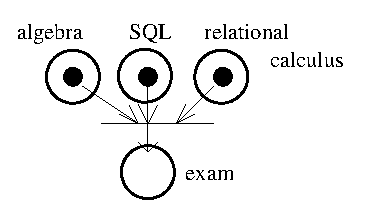
\includegraphics[width=45mm]{petria.eps}
\caption{Egt specification (SQL chapters) (A).}
\label{petria}
\end{center}
\end{figure}


In order to model e-learning guided tours (egt), we choose
hierarchical colour Petri nets~\cite{Petri}. Figure~\ref{petria}
illustrates a Petri net for representing an egt through SQL exercises
at the chapter level according to the aforementioned scenario. This
egt specifies that any student has to first 
train through exercises on relational algebra, SQL and relational
calculus in any order prior to taking an exam on SQL. With each
student is associated a coloured token. The firing of the SQL
transition is performed only when the student is in the final place of
the lower level Petri net (figure~\ref{petrib}). Thus, the Petri net
figure~\ref{petrib} refines the place called SQL in the Petri net figure~\ref{petria}. This Petri net \ref{petrib} specifies
that to pass this step, the student has to perform 3 out of 10
exercices. Note that the firing of an elementary transition 
(exercise performed) is
not specified here. It might be answering the questions of the
exercises (the insertion of this event in the student log, see
following subsection, might trigger the transition), it might be a
stronger condition, such as successfully answering the exercises (the
latter process implying a manual or automatic correct answer mechanism
with a possible interaction with the teacher, which process when
terminated corresponds as well to the insertion of an item in the
student log which item triggers the transition).

\begin{figure}[htbp]
\begin{center}
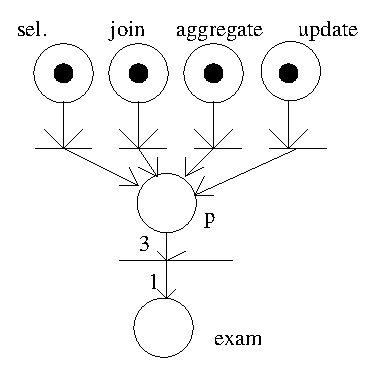
\includegraphics[width=45mm]{petrib.eps}
\caption{Egt specification (relational algebra) (B).}
\end{center}
\label{petrib}
\end{figure}


Three remarks are noteworthy:

\begin{enumerate}

  \item the specification process of the hierarchical Petri net like
  egt is very general and only assumes a hierarchical structuring of
  the document and an egt per level: at each level the egt generation
  is parametrized by (it takes as an entry) the e-learning material
  structure (DTD) as well as the teacher specifications.

  \item It is also important to note that displaying at each level the
  Petri net with tokens of a given colour or with a counter on the
  number of tokens in a given place allows for snapshots on the state
  of progress of a given student, respectively of a set of students.

  \item the above egt specification is based on the past history of a
  given student. One might as well specify egt according to other
  criteria, such as different \emph{a priori} levels of students,
  multi-pedagogical targets (the same bank of sharable course or
  exercises documents might be shared among various e-learning
  situations, actors and targets).
\end{enumerate}

\subsection{Student Log}

Each student action is recorded in a log and identified by the log
item number. The objective is two-fold: first the egt for a student is
dependent on his/her current state (and possibly on his/her past
actions) which has then to be recorded. Second our objective is to
keep track of all student actions at some level of abstraction for
further data mining. 
%AM I think the following lines may be left out here.
%As specified in the section on data mining,
%keeping track of student actions might be necessary to better
%understand the learning behavior of a given set of students, to
%improve the e-learning process and more specifically here to improve
%the guided tours through a given set of learning documents, or
%possibly to modify the structure and contents of these e-learning
%materials.

With each student action (basically accessing in read mode a course
item, answering in write mode an exercise) corresponds a log item to
be inserted into the database. This insertion might trigger a change of
state i.e; the firing of a transition in a egt. The actual structure
of the database (the log item) depends on the data mining targets as
well as on the e-learning situation. However it should include the
following attributes:

\begin{itemize}
\item item id
\item student id
\item identification of the piece of document (node or leaf) accessed
\item access time and duration
\item access mode (read only, write, etc.)
\item if the mode is write, answer text
\item if the mode is write with answer
  \begin{itemize}
  \item  grade obtained,
  \item  mistakes types,
  \end{itemize}
\item  if the mode is write with comment, customized teacher comment
  according to the answer,
etc.
\end{itemize}

Two remarks are noteworthy.

\begin{enumerate}

  \item Using standard database querying on sequences of log items,
  one might obtain some aggregated information on grades, duration and
  higher level nodes accessed (simple extensions of database query
  standards allow to understand that if a node on selection is
  accessed, then a node on relational algebra has been accessed). An
  example of such a query is ``get the number of exercises on
  relational algebra performed by Naomi between day d and day d', the
  duration and the sum of grades for these exercises''.

  \item It is not our purpose to completely specify the information
  system behind the student log. For example in an alternate design,
  one could distinguish between student items in the log (one per
  action) and subsequent teacher items on a given student action such
  as giving a customized feedback or just a grade. In the latter case,
  the teacher item should include the student action id (log id) as a
  foreign key. In that case the firing of a place might be triggered
  not by the insertion in the log of the student action but by the
  insertion of the subsequent teacher action.

\end{enumerate}

\subsection{Functional architecture}

The three above information components suggest the existence of the
following software components: 1) student interface, or e-learning
guided tour, for accessing to and navigating through e-learning
material; 2) authoring interface for specifying an egt, 3) tutor
interface for (a) querying the current state of the system and (b) for
data mining. Other components are necessary as well which are not even
sketched here. These include a model for exercise answering and
methods and code for response analysis. We end up the section by
briefly describing the three above components.

\subsubsection*{Student interface}

The learner interface, or e-learning guided tour (egt), includes a
general interface allowing to display the offer and structure of
available course material and the interface allowing to access and
answer e-learning material according to the egt and the student
history. This interface relies on the underlying hierarchical Petri
net model for egt.


\subsubsection*{Authoring interface}

The Authoring interface allows specifying egt. Starting from the
structure (XML schemas) of the e-learning items the author specifies
the constraints on the access to items (interdiction, inclusive or,
and, conditions on numbers, etc.) as illustrated on the examples
above. A graphical user interface helps the author to specify these
constraints which expressiveness is that of the underlying couloured
Petri net model.

\subsubsection*{Data miner and visualizer}

Author interface for querying the state of progress and data mining
the students works.  Standard relational queries on the database
(including the student log) allow for snapshots and history of the
student(s) progress in the e-learning process. The Petri net
underlying modelling allows for identifying individual and group
behaviours in the event driven e-elarning process. As alreeady
suggested, one can visualize and summarize where the students
currently stand (in which places they currently are). Keeping track of
all student (and teacher actions) allow for subsequent mining as
detailed in the last section. It is worth noticing that keeping track of
the complete navigation through the e-learning material allows not
only the mining of elementary actions but more important of chains of
actions in time (complete tours through the e-learning
material).




